% !TEX encoding = UTF-8 Unicode 
\documentclass[9pt, aspectratio=169, xcolor=table]{beamer}
\setbeamercovered{transparent=10}
\usetheme[
%  showheader,
  colorblocks,
%  noframetitlerule,
]{Verona}
\definecolor{deepbullblue}{rgb}{0,0.298, 0.427}
\definecolor{sunbeltyellow}{rgb}{1,0.792, 0.024}
\definecolor{redbullred}{rgb}{0.8,0.122, 0.294}
\definecolor{mGreen}{rgb}{0,0.6,0}
\definecolor{mGray}{rgb}{0.5,0.5,0.5}
\definecolor{grissuave}{rgb}{0.25,0.25,0.25}
\definecolor{mPurple}{rgb}{0.58,0,0.82}
\definecolor{backgroundColour}{rgb}{0.95,0.95,0.92}

\definecolor{alizarin}{rgb}{0.82, 0.1, 0.26}
\definecolor{ao}{rgb}{0.0, 0.5, 0.0}

\usepackage{minted}
\usepackage{svg}
\usepackage{listings}

\usepackage[spanish,es-tabla]{babel}

\lstdefinestyle{CStyle}{
    backgroundcolor=\color{backgroundColour},   
    commentstyle=\color{mGreen},
    keywordstyle=\color{magenta},
    numbers=none,
    %numberstyle=\tiny\color{mGray},
    %numbers=left,                    
    %numbersep=5pt,                  
    stringstyle=\color{mPurple},
    basicstyle=\ttfamily,
    breakatwhitespace=false,         
    breaklines=true,                 
    captionpos=b,                    
    keepspaces=true,                 
    showspaces=false,
    columns=fixed,
    showstringspaces=false,
    showtabs=false,                  
    tabsize=2,
    language=C
}

\usepackage[T1]{fontenc}
\usepackage[utf8]{inputenc}
\usepackage{listings}
\usepackage{datetime}
\usepackage{lipsum}
\usepackage{todonotes}
\usepackage[export]{adjustbox}
%\usepackage[spanish,onelanguage,boxed, boxruled, algoruled]{algorithm2e}
%\usepackage[spanish,onelanguage,boxed, algoruled]{algorithm2e}
%\usepackage{algcompatible}
\usepackage{algorithm}
\usepackage[noend]{algpseudocode}
%%%%%%%%%%%%%%%%%%%%%%%%%%%%%%%
% Mac上使用如下命令声明隶书字体,windows也有相关方式,大家可自行修改
%\providecommand{\lishu}{\CJKfamily{zhli}}
%%%%%%%%%%%%%%%%%%%%%%%%%%%%%%%
\usepackage{tikz}
\usetikzlibrary{fadings}
%
%\setbeamertemplate{sections/subsections in toc}[ball]
%\usepackage{xeCJK}
\usepackage{caption}
\usepackage{subcaption}
\usefonttheme{professionalfonts}
\def\mathfamilydefault{\rmdefault}
\usepackage{amsmath}
%\setlength{\mathindent}{0pt}
\usepackage{multirow}
\usepackage{booktabs}
\usepackage{multicol}
\usepackage{bm}

\def\testclr#1#{\@testclr{#1}}
%\def\@testclr#1#2{\scalebox{0.7}{\colorbox#1{#2}{\phantom{X}}}}
\def\@testclr#1#2#3{{\colorbox#1{#2}{#3}}}

\setbeamertemplate{section in toc}{\hspace*{1em}\inserttocsectionnumber.~\inserttocsection\par}
\setbeamertemplate{subsection in toc}{\hspace*{2em}\inserttocsectionnumber.\inserttocsubsectionnumber.~\inserttocsubsection\par}
\setbeamerfont{subsection in toc}{size=\small}

\title{AMMM - Course project}
\subtitle{Master in Research and Innovation in Informatics}
\author[Ignacio Encinas Rubio, Adrián Jiménez González]{Ignacio Encinas Rubio, Adrián Jiménez Gonzalez}
\mail{\{ignacio.encinas,adrian.jimenez.g\}@estudiantat.upc.edu}
\institute[]{Polytechnic University of Catalonia}
\date{\today}
\titlegraphic[width=3.5cm]{logo_upc.png}{}

\usepackage{tcolorbox}
\usepackage{fontawesome}

\begin{document}


\maketitle

%%% define code
\defverbatim[colored]\lstI{
	\begin{lstlisting}[language=C++,basicstyle=\ttfamily,keywordstyle=\color{red}]
	int main() {
	// Define variables at the beginning
	// of the block, as in C:
	CStash intStash, stringStash;
	int i;
	char* cp;
	ifstream in;
	string line;
	[...]
	\end{lstlisting}
}
%%%%%%%%%%%%%%%%%%%%%%%%%%%%%%%%
% ----------- FRAME ------------
%%%%%%%%%%%%%%%%%%%%%%%%%%%%%%%%
\begin{frame}%
	\frametitle{Contents}%
	%\textbf{\tableofcontents[currentsection]} %
	\begin{columns}[t]
	    \begin{column}{.5\textwidth}
		\tableofcontents[sections={1-2}]
	    \end{column}
	    \begin{column}{.5\textwidth}
		\tableofcontents[sections={3-5}]
	    \end{column}
	\end{columns}
\end{frame}%

\section{Problem Statement}
\begin{frame}{\secname}
    \begin{tcolorbox}[colback=gray!30, colframe=Veronablue, arc=0pt, outer arc=0pt, title = \textbf{Main requirements}]
    \begin{enumerate}
	\item Each contestant will play exactly once against each of the other contestants.
	\item Each round will consist of $\frac{n-1}{2}$ matches.
	\item Players will play 50\% of their games as white, 50\% will be played as black.
    \end{enumerate}
    \end{tcolorbox}

    \begin{tcolorbox}[colback=gray!30, colframe=Veronablue, arc=0pt, outer arc=0pt, title = \textbf{Subtle requirements}]
    \begin{itemize}
	\item A player can only play up to 1 game per round
	\item A player can't play against himself
    \end{itemize}
    \end{tcolorbox}
    
\end{frame}

\subsection{Inputs \& Outputs}
\begin{frame}{\secname: \subsecname}
    \begin{tcolorbox}[colback=gray!30, colframe=Veronablue, arc=0pt, outer arc=0pt, title = \textbf{Inputs}]
    \begin{itemize}
	\item Number of contestants, $n$. Has to be odd
	\item Matrix of points per day per player, $p_{n \times n}$
    \end{itemize}
    \end{tcolorbox}

    \begin{tcolorbox}[colback=gray!30, colframe=Veronablue, arc=0pt, outer arc=0pt, title = \textbf{Outputs}]
    \begin{itemize}
	\item Schedule with the set of pairings \{\{$r_1$, $p_i$, $p_j$\}, \dots, \{$r_n$, $p_k$, $p_h$\}\} that maximizes total score. Ensured to be optimal if it's obtained through the ILP.
    \end{itemize}
    \end{tcolorbox}
    
\end{frame}

\subsection{Definitions}
\begin{frame}{\secname: \subsecname}
    In order to specify the constraints, we need to specify the sets and variables we're going to work with:
    \vspace{1cm}

    \begin{minipage}{0.49\textwidth}
	\begin{itemize}
	    \item $M(x, y)$ matches played among $x$ and $y$ (\textcolor{Veronablue}{1})
	    \item $R(r)$  matches played at round $r$ (\textcolor{Veronablue}{2})
	    \item $W(p)$ matches played by player $p$ as white (\textcolor{Veronablue}{3})
	    \item $B(p)$ matches played by player $p$ as black (\textcolor{Veronablue}{3})
	    \item $G(p,r)$ games played by $p$ at round $r$ (\textcolor{Veronablue}{4})
	    \item $F(r)$ free players at round $r$ (\textcolor{Veronablue}{5})
	\end{itemize}
    \end{minipage}
    \hfill
    \begin{minipage}{0.49\textwidth}
	\begin{enumerate}
	    \item Each contestant will play exactly once against each of the other contestants.
	    \item Each round will consist of $\frac{n-1}{2}$ matches.
	    \item Players will play 50\% of their games as white, 50\% will be played as black.
	    \item Players can play up to 1 match per round
	    \item Objective function
	\end{enumerate}
    \end{minipage}
    
\end{frame}

\section{Integer Linear Programming Model}
\subsection{Variables}
\begin{frame}{\secname: \subsecname}
    Every set will be constructed from a boolean multidimensional array. \textit{m}$[w][b][r]$ will be 1 whenever player $w$ plays player $b$ in round $r$, and 0 otherwise.
    \begin{tcolorbox}[colback=gray!30, colframe=Veronablue, arc=0pt, outer arc=0pt, title = \textbf{Set constructions}]
	\begin{align*}
	    M(x, y)   &= \{\{x, y, r\}, &\ r \in [1, Rounds]              \ &| \ \text{m}[x][y][r] = 1 \lor \text{m}[y][x][r] = 1                         &\}\\
	    F(r)      &= \{p          , &\ p \in [1, n]                   \ &| \ \text{m}[p][o][r] = 0 \land \text{m}[o][p][r] = 0  \quad \forall o \in [1, n]&\}\\
	    W(p)      &= \{\{p, b, r\}, &\ r \in [1, Rounds], b \in [1, n]\ &| \ \text{m}[p][b][r] = 1                                                    &\}\\
	    B(p)      &= \{\{w, p, r\}, &\ r \in [1, Rounds], w \in [1, n]\ &| \ \text{m}[w][p][r] = 1                                                    &\}\\
	    R(r)      &= \{\{w, b, r\}, &\ w, b \in [1, n]                \ &| \ \text{m}[w][b][r] = 1                                                    &\}\\
	    G(p, r)   &= \{\{o, p, r\}, &\ o \in [1, n]                   \ &| \ \text{m}[p][o][r] = 1  \lor \text{m}[o][p][r] = 1                        &\}\\
	\end{align*}
    \end{tcolorbox}
\end{frame}

\subsection{Constraints}
\begin{frame}{\secname: \subsecname}
    \begin{minipage}{0.49\textwidth}
	\begin{equation}
	    \label{playwitheachother}
	    |M(x,y)| = 1 \quad \forall x,y \in P \ | \  x \neq y
	\end{equation}

	\begin{equation}
	    \label{matchesperround}
	    |R(r)| = \frac{n-1}{2}  \quad \forall r \in [1,\ \text{Rounds}] 
	\end{equation}

	\begin{equation}
	    \label{fairness}
	    |W(p)| = \frac{n-1}{2} \quad \forall p \in P
	\end{equation}

	\begin{equation}
	    \label{1gameperround}
	    |G(p,r)| \leq 1 \quad \forall p \in P, r \in [1, \ \text{Rounds}] 
	\end{equation}


    \end{minipage}
    \hfill
    \begin{minipage}{0.49\textwidth}
	\begin{enumerate}
	    \item Each contestant will play exactly once against each of the other contestants.
	    \item Each round will consist of $\frac{n-1}{2}$ matches.
	    \item Players will play 50\% of their games as white, 50\% will be played as black.
	    \item Players can play up to 1 match per round
	\end{enumerate}
    \end{minipage}

\end{frame}

\subsection{Redundant constraints}
\begin{frame}{\secname: \subsecname}
    \begin{minipage}{0.40\textwidth}
	Redundant constraints might appear to make the model faster but they seem make it slower in the long run
	\begin{equation*}
	    \label{noselfplay}
	    |M(x,x)| = 0 \quad \forall x \in P 
	\end{equation*}

	\begin{equation*}
	    \label{blackfairness}
	    |B(p)| = \frac{n-1}{2} \quad \forall p \in P
	\end{equation*}

    \end{minipage}
    \hfill
    \begin{minipage}{0.57\textwidth}
	\begin{figure}[h]
	    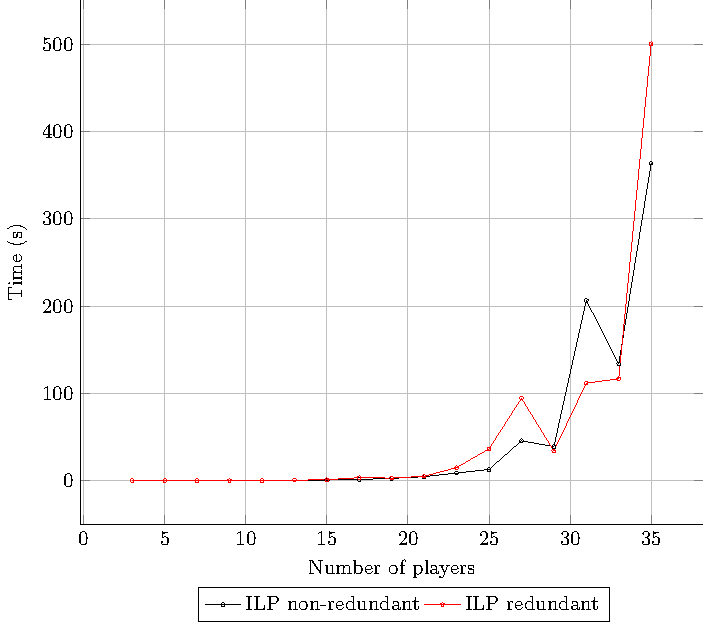
\includegraphics[width=\linewidth]{../plots/time_per_instance.pdf}
	\end{figure}
    \end{minipage}

\end{frame}

\section{Metaheuristics}
\subsection{Greedy algorithm}
\begin{frame}{\secname: \subsecname}
\begin{tcolorbox}[colback=gray!30, colframe=Veronablue, arc=0pt, outer arc=0pt, title = \textbf{Greedy cost function}]
    \begin{equation*}
      q(c,day)= c.points\_per\_day[day]
    \end{equation*}
\end{tcolorbox}


\begin{algorithm}[H]
	\caption{Greedy algorithm} 
	\begin{algorithmic}[1]
	  \State Players $\leftarrow$ Set of Players
	  \State rests $\leftarrow$ \{\}
	  \For {day in 0..days}
	    \State playersToRest $\leftarrow$ filter Players(p) $|$ p.hasNotRested
	    \State sortedPlayers $\leftarrow$ sort playersToRest(p) by q(p,day) (DESC) 
	    \State rests[day]\ $\leftarrow$\ sortedPlayers.first()
	  \EndFor
	\end{algorithmic} 
\end{algorithm}
\end{frame}

\subsection{Local Search}
\begin{frame}{\secname: \subsecname}
\begin{algorithm}[H]
	\caption{Local Search} 
	\begin{algorithmic}[1]
    \For {i in 0..days}
    \State best\_swap\_points $\leftarrow$ 0
    \State best\_swap $\leftarrow$ i
      \For {j in 0..days}
        \State change = EvaluateRestSwap(i,j)
        \If{change $>$ best\_swap\_points}
          \State best\_swap\_points $\leftarrow$ change
          \State best\_swap $\leftarrow$ j
        \EndIf
      \EndFor
      \State rests[i] $\leftrightarrow$ rests[best\_swap]
		\EndFor
	\end{algorithmic} 
\end{algorithm}



\end{frame}

\subsection{GRASP}
\begin{frame}{\secname: \subsecname}
\begin{algorithm}[H]
    \caption{constructRCL(day)} 
    \label{rcl}
    \begin{algorithmic}[1]
	\State $q_{max} \leftarrow $ sortedPlayers.first().points[d]
	\State $q_{min} \leftarrow$ sortedPlayers.last().points[d]
	\State $RCL_{max}$ $\leftarrow$ $\{p \in sortedPlayers\ |\ p.points[d] >= q_{max} - \alpha \cdot (q_{max} - q_{min})\}$
    \end{algorithmic} 
\end{algorithm}




\begin{algorithm}[H]
	\caption{GRASP} 
	\begin{algorithmic}[1]
	  \State rests $\leftarrow$ \{\}
	    \For {day in 0..days}
        \State playersToRest $\leftarrow$ filter Players(p) $|$ p.hasNotRested
        \State sortedPlayers $\leftarrow$ sort playersToRest(p) by q(p,day) (DESC)
	      \State RCL $\leftarrow$ constructRCL(day)
	      \State select p $\in$ RCL randomly
	      \State rests[day]\ $\leftarrow$\ p
	    \EndFor
	\end{algorithmic} 
\end{algorithm}
\end{frame}

\subsubsection{Parameter tuning}
\begin{frame}{\subsecname: \subsubsecname}

    \begin{minipage}{0.44\textwidth}
	\begin{itemize}
	    \item Figure shows the arithmetic mean error with respect to the optimal solution for each of the instances.
      \item We keep the smallest alpha that gives the minimum mean error.
	\end{itemize}
    \end{minipage}
    \hfill
    \begin{minipage}{0.52\textwidth}
	\centering
	\begin{figure}[H]
	    \centering
	    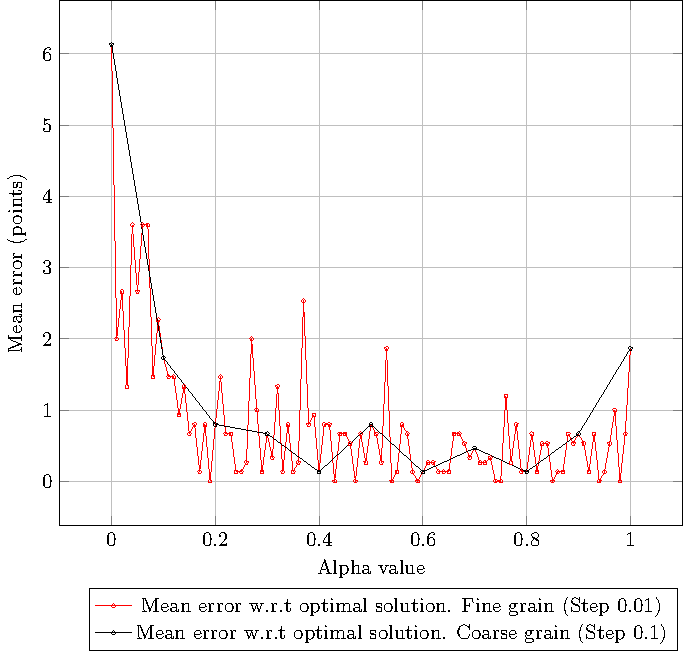
\includegraphics[width=\linewidth]{../plots/error.pdf}
	    \label{fig:error}
	\end{figure}
    \end{minipage}
\end{frame}

\section{Results}
\subsection{Time}
\begin{frame}{\secname: \subsecname}
    \begin{minipage}{0.44\textwidth}
	\begin{itemize}
	    \item Greedy and Local Search need approximately same time to reach the solution. They're fastest but their quality of the solution is too low.
	    \item GRASP sacrifices some runtime performance to improve the quality of the solution.
      \item ILPs obtain the optimal solution at cost of being several orders of magnitude slower due to the complexity of creating valid pairings.
      \item ILP rest obtains the optimal solution just computing the rest day for each player. It is not much slower than GRASP and for large instances it can be even faster.
	\end{itemize}
    \end{minipage}
    \hfill
    \begin{minipage}{0.52\textwidth}
	\centering
	\begin{figure}[H]
	    \centering
	    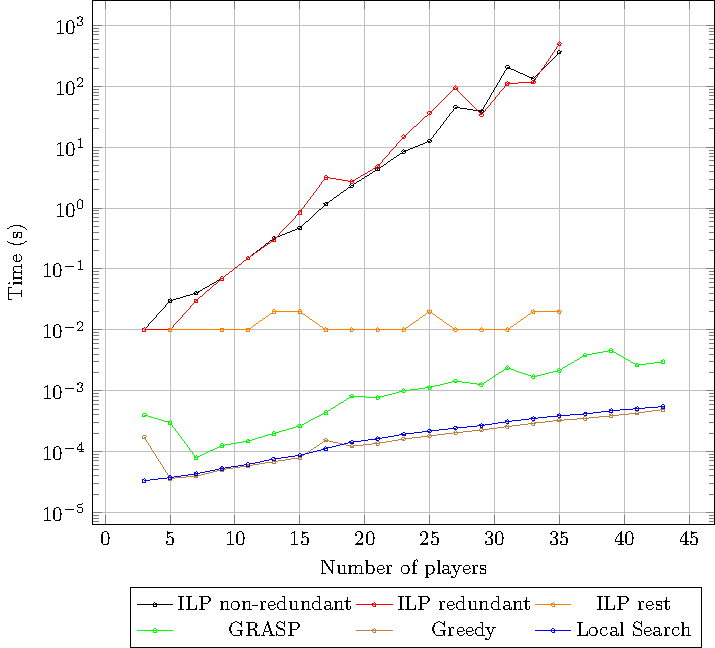
\includegraphics[width=\linewidth]{../plots/times.pdf}
	\end{figure}
    \end{minipage}
\end{frame}

\subsection{Quality of solutions}
\begin{frame}{\secname: \subsecname}
    \begin{minipage}{0.44\textwidth}
	\begin{itemize}
	    \item Greedy offers the worst solution for every instance
	    \item Greedy + Local Search improves the quality of the solution taking practically the same time as Greedy.
      \item GRASP commonly reachs the optimal solution, having a good improvement over Local  Search.
	\end{itemize}
    \end{minipage}
    \hfill
    \begin{minipage}{0.52\textwidth}
	\centering
	\begin{figure}[H]
	    \centering
	    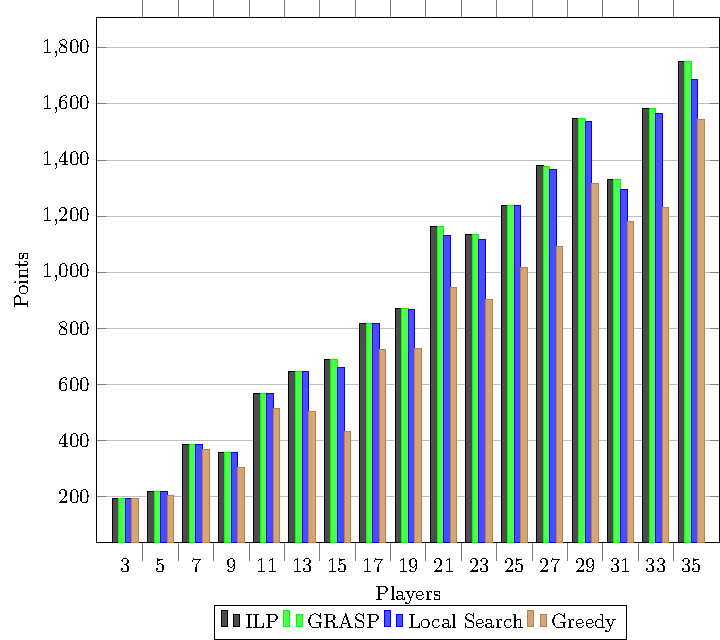
\includegraphics[width=\linewidth]{../plots/solutions.pdf}
	\end{figure}
    \end{minipage}
\end{frame}

%\begin{frame}[noframenumbering]{\secname}

%\end{frame}


\end{document}
